\documentclass[12pt, twoside]{article}
\usepackage[letterpaper, margin=1in, headsep=0.2in]{geometry}
\setlength{\headheight}{0.6in}
%\usepackage[english]{babel}
\usepackage[utf8]{inputenc}
\usepackage{microtype}
\usepackage{amsmath}
\usepackage{amssymb}
%\usepackage{amsfonts}
\usepackage{siunitx} %units in math. eg 20\milli\meter
\usepackage{yhmath} % for arcs, overparenth command
\usepackage{tikz} %graphics
\usetikzlibrary{quotes, angles}
\usepackage{graphicx} %consider setting \graphicspath{{images/}}
\usepackage{parskip} %no paragraph indent
\usepackage{enumitem}
\usepackage{multicol}
\usepackage{venndiagram}

\usepackage{fancyhdr}
\pagestyle{fancy}
\fancyhf{}
\renewcommand{\headrulewidth}{0pt} % disable the underline of the header
\raggedbottom
\hfuzz=2mm %suppresses overfull box warnings

\usepackage{hyperref}

\fancyhead[LE]{\thepage}
\fancyhead[RO]{\thepage \\ Name: \hspace{4cm} \,\\}
\fancyhead[LO]{BECA / Dr. Huson / Geometry\\*  Unit 1: Segments, length, and area\\* 23 Sept 2022}

\begin{document}

\subsubsection*{1.12 Extension unit test: Confidence intervals, absolute value, scientific notation}
\begin{enumerate}
\item Given $\overline{ABC}$, $AB=1 \frac{5}{6}$, and $AC=6 \frac{1}{3}$. Find ${BC}$. \par \bigskip
\begin{tikzpicture}
  \draw[thick] (1,0)--(7,0);
  \draw[fill] (1,0) circle [radius=0.05] node[below]{$A$};
  \draw[fill] (2.5,0) circle [radius=0.05] node[below]{$B$};
  \draw[fill] (7,0) circle [radius=0.05] node[below]{$C$};
\end{tikzpicture} \vspace{1cm}

\item Round each value to three sig figs
\begin{multicols}{2}
  \begin{enumerate}
    \item 20,201,249 \par \medskip (population of New York State)
    \item 21,538,187 \par \medskip (population of Florida)
  \end{enumerate}
\end{multicols}

\item During COVID, New York Governor Cuomo criticized Florida Governor DeSantis, saying that Florida had more deaths than NY. What is the relative difference in population between the states expressed as a percentage? (i.e. \% error by assuming NY actually has as many people as FL) \vspace{2cm}

\item Given $x=-4$ simplify each expression. (try to do them without a calculator)
\begin{multicols}{2}
  \begin{enumerate}[itemsep=1.25cm]
    \item $|2+x|=$
    \item $|2-x|=$
    \item $|x|-|x|=$
    \item $2 |x+3|-2x=$
  \end{enumerate}
\end{multicols} \vspace{1cm}

\item Find all values of $x$ satisfying the equation. (show the two cases and checks) 
$$ 5|x+3|-12 = 18$$

\newpage
\item The length of a piece of lumber is 96 inches plus or minus 1 inch. Express the length of the board in centimeters in the form $l \pm \epsilon$. \vspace{3cm}

\item The earth's moon is approximately 238,900 miles from our planet. 
\begin{enumerate}
  \item Find the circumference of its orbit rounded to the \emph{nearest thousand} miles. (assume a circular orbit) \vspace{1cm}
  \item Convert the result to scientific notation rounded to three sig figs
\end{enumerate} \vspace{1cm}

\item The dimensions of a rectangular sheet of plywood are 4 feet by 8 feet. Each length is accurate plus or minus one inch. Find the area of the plywood in square feet, rounded to three significant figures. Express the answer as an interval. \vspace{3cm}

\item A rectangle is 10 centimeters longer than it is wide. Given that its perimeter is $80 \text{ cm}^2$, find its \emph{area}. 
  \begin{flushleft}
  \begin{tikzpicture}[scale=0.8]
    \draw[thick] (0,0)--(6,0)--(6,3.5)--(0,3.5)--cycle;
    \node at (3,-0.8){$x + 10$ cm};
    \node at (6.8,2.3){$x$};
    \draw (2.9, -0.2)--(2.9,0.2);
    \draw (2.9, 3.3)--(2.9,3.7);
    \draw (-0.2, 1.9)--(0.2, 1.9);
    \draw (-0.2, 1.7)--(0.2, 1.7);
    \draw (5.8, 1.9)--(6.2, 1.9);
    \draw (5.8, 1.7)--(6.2, 1.7);
    \end{tikzpicture}
  \end{flushleft} \vspace{4cm}

\newpage
\item A thin rectangular strip with width $w=5$ is shown on top of a larger square, below.
  \begin{multicols}{2}
    \begin{tikzpicture}[rotate=90]
      \draw[thick] (0,0) rectangle (5.5,4);
      \draw[thick] (4,0) -- (4,4);
      \node at (4.7,-0.4){5};
    \end{tikzpicture}
    \begin{enumerate}
      \item The perimeter of the square is 64. Find the area of the square. \vspace{2cm}
      \item Find the area of the thin rectangle on top.
      \end{enumerate}
    \end{multicols}
  
\emph{All algebraic solutions require a check for full credit.}
\item Given that $M$ is the midpoint of segment $\overline{AB}$, $AM=\frac{2}{3}(6x+9)$ and $AB=28$.
  Find $x$.
  \begin{flushleft}
    \begin{tikzpicture}[scale=1]
      \draw[thick] (0,0)--(8,0);
      \draw[fill] (0,0) circle [radius=0.05] node[below]{$A$};
      \draw[fill] (4,0) circle [radius=0.05] node[below]{$M$};
      \draw[fill] (8,0) circle [radius=0.05] node[below]{$B$};
      \node at (2,0.7){$\frac{2}{3}(6x+9)$};
      \draw[<->, dashed] (0,-1)--(8,-1);
      \node at (4,-1.5){$28$};
      \draw (1.8,-0.2)--(1.9,0.2);
      \draw (2.1,-0.2)--(2.2,0.2);
      \draw (5.8,-0.2)--(5.9,0.2);
      \draw (6.1,-0.2)--(6.2,0.2);
    \end{tikzpicture}
  \end{flushleft} \vspace{4cm}

\item The isosceles $\triangle RST$ has a perimeter measuring 75. Given $RS=RT=5x+4$ and $ST=17$, find $x$.  \par \smallskip
  \begin{tikzpicture}[scale=0.7,rotate=110]
    \draw[thick](0,0)--(4,0)--(2,6)--(0,0);
    \draw[fill] (0,0) circle [radius=0.05] node[below]{$S$};
    \draw[fill] (4,0) circle [radius=0.05] node[right]{$T$};
    \draw[fill] (2,6) circle [radius=0.05] node[above left]{$R$};
    \draw[thick] (0.8,3.1)--(1.2,3); %tick mark
    \draw[thick] (2.8,3)--(3.2,3.1); %tick mark
    \node at (2,0) [right]{$17$};
    \node at (0.8,3.4) [below]{$5x+4$};
  \end{tikzpicture} \vspace{3cm}
  

\newpage
\item Point $M=(1.7)$ is the midpoint of $P=(-2.5)$ and $Q$, as shown on the number line. Find the value of $Q$. Mark and label it below. \par \medskip
  \begin{tikzpicture}
    \draw[<->] (-3.5,0)--(7.5,0);
    \foreach \x in {-3,...,7}
      \draw[shift={(\x,0)},color=black] (0pt,-3pt) -- (0pt,3pt) node[below=5pt]  {$\x$};
    \draw[fill] (-2.5,0) circle [radius=0.05] node[above]{$P(-2.5)$};
    \draw[fill] (1.7,0) circle [radius=0.05] node[above]{$M(1.7)$};
  \end{tikzpicture} \vspace{3cm}

\item Four identical circles touch but do not overlap, as shown. Their total area is $49\pi$. Find the common radius $r$. \par
  \begin{tikzpicture}[scale=0.4]
    %\draw[help lines] (0,0) grid (10,8);
    \draw[thick, ->] (-1.2,0) -- (15.4,0) node [above right]{$x$};
    \draw[thick, ->] (0,-1.2)--(0,15.4) node [above right]{$y$};
    \foreach \x in {2,4,...,14}
      \draw[shift={(\x,0)}] (0pt,-3pt)--(0pt,3pt) node[below=5pt]{$\x$};
    \foreach \y in {2,4,...,14}
      \draw[shift={(0,\y)}] (-3pt,0pt)--(3pt,0pt) node[left=5pt]{$\y$};
    \draw[thick] (4,4) circle [radius=3.5];
    \draw[thick] (11,4) circle [radius=3.5];
    \draw[thick] (4,11) circle [radius=3.5];
    \draw[thick] (11,11) circle [radius=3.5];
    \fill (11,4) circle [radius=0.15];
    \draw[<->,dashed, shift={(11.1,4.05)}] (0,0)--(27:3.3);
    \node at (13,4){$r=?$};
  \end{tikzpicture} \vfill

\subsubsection*{Academic integrity pledge}
This assignment must be completed in one sitting. Use your notes and a calculator. \par \smallskip
I have not received any human help on this assignment. \par \bigskip
Signed: \rule{6cm}{0.15mm} \hfill \rule{6cm}{0.15mm}
\begin{flushright}
  Date, start time - end time
\end{flushright}
  

\end{enumerate}
\end{document}